\documentclass[11pt]{article}

% { BEGIN_FOLD -----------PACKAGES------------
\usepackage[mathscr]{euscript}

\newcommand\subheading[2]{\vspace{.25in}\hrule\textbf{#1: #2}\vspace{.5em}\hrule\vspace{.10in}}
\renewcommand\part[1]{\vspace{.10in}\textbf{(#1)}}

\usepackage{amsmath, amssymb, amsthm} %AMS packages
\usepackage{mathtools, graphicx, enumitem} %generally recommended
\usepackage{mathrsfs} %symbols I like
\usepackage{hyperref} %personal preference
\usepackage{microtype, } %recommended by stackexchange, never tried them myself
\usepackage{bigints}
\theoremstyle{definition}
\newtheorem{definition}{Definition}[section]
\newtheorem{theorem}{Theorem}

% Layout
\usepackage{fancyhdr}
\usepackage[margin=1in]{geometry}
\lhead{}
\chead{}
\rhead{PRUV 2023}
\setlength{\parindent}{0pt}
\setlength{\parskip}{5pt plus 1pt}
\setlength{\headheight}{13.6pt}
\pagestyle{fancyplain}

\setlist[itemize]{noitemsep}
\setlist[enumerate]{noitemsep}

%-------------------------------------------<commands>--------------------------------------------------------
%%%%%%%%%%%%%%%%%%%%%%%%%%%%%%%%%%%%%%%%%											Letter Symbols
\newcommand{\R}{\mathbb{R}}
\newcommand{\N}{\mathbb{N}}
\newcommand{\Z}{\mathbb{Z}}
\newcommand{\Q}{\mathbb{Q}}
\newcommand{\C}{\mathbb{C}}
\newcommand{\F}{\mathcal{F}}
\renewcommand{\P}{\mathbb{P}} %overwrites pilcrow
\renewcommand{\H}{\mathcal{H}} %overwrites long-umlaut diacritic
\newcommand{\eps}{\varepsilon}
\newcommand{\E}{\mathbb{E}}
%%%%%%%%%%%%%%%%%%%%%%%%%%%%%%%%%%%%%%%%%											Brackets
\newcommand{\paren}[1]{\left( #1 \right)}
\newcommand{\bracket}[1]{\left[ #1 \right]}
\newcommand{\chevron}[1]{\langle #1 \rangle}
\newcommand{\norm}[2][ ]{\left\lVert #2 \right\rVert_{#1}} % optional argument for subscript
\newcommand{\abs}[1]{\left\lvert #1 \right\rvert}
\newcommand{\floor}[1]{\left\lfloor #1 \right\rfloor}
\newcommand{\ceil}[1]{\left\lceil #1 \right\rceil}
%%%%%%%%%%%%%%%%%%%%%%%%%%%%%%%%%%%%%%%%%											Operators
\DeclareMathOperator{\supp}{supp} % support
\DeclareMathOperator{\trace}{tr}
\DeclareMathOperator{\lspan}{span}
\DeclareMathOperator{\conv}{conv} % stands for conv, as in convex hull
\DeclareMathOperator{\Int}{int} % stands for int, as in interior of a set
\DeclareMathOperator{\cl}{cl} % closure
\DeclareMathOperator{\sgn}{sgn}
%%%%%%%%%%%%%%%%%%%%%%%%%%%%%%%%%%%%%%%%%%											Arrows
\newcommand{\into}{\hookrightarrow} % injection
\newcommand{\onto}{\twoheadrightarrow} % surjection
\newcommand{\unif}{\righrightarrows} % uniform convergence
\newcommand{\weakly}{\rightharpoonup} % weak convergence
\newcommand{\isom}{\cong} % isometry (not technically an arrow)
\newcommand{\restr}[1]{{\upharpoonright}_{#1}} % function restriction
%%%%%%%%%%%%%%%%%%%%%%%%%%%%%%%%%%%%%%%%%%											Common Abbreviations
\renewcommand{\th}{^\mathrm{th}} %overwrites thorn (old english letter)
\newcommand{\n}{^{-1}}
\newcommand{\half}{\frac{1}{2}}
%%%%%%%%%%%%%%%%%%%%%%%%%%%%%%%%%%%%%%%%%%											Differential Operators
\newcommand{\del}{\partial}
\newcommand{\grad}{\nabla}
\newcommand{\Laplace}{\Delta}
\renewcommand{\div}{\operatorname{div}} %overwrites division symbol
\newcommand{\dd}{\mathrm{d}}
\newcommand{\intd}{\,\dd}
\newcommand{\ddt}{\frac{\dd}{\dd t}}
\newcommand{\deriv}[2]{\frac{\dd #1}{\dd #2}} %can leave top blank, e.g. \deriv{}{x}
\newcommand{\pderiv}[2]{\frac{\partial #1}{\partial #2}} %ditto
%%%%%%%%%%%%%%%%%%%%%%%%%%%%%%%%%%%%%%%%%%											Favorite Functions and Space Names
\newcommand{\test}{\mathcal{D}}
\newcommand{\Ctest}{C_c^\infty}
\newcommand{\BMO}{\operatorname{BMO}}
\newcommand{\indic}[1]{\chi_{\{#1\}}}
\newcommand{\Leb}[2][\R^n]{L^{#2}(#1)} % L^p space
%-------------------------------------------</commands>--------------------------------------------------------
% }  -----------PACKAGES------------

\title{Testing for Geometry in 2-Parameter Random Simplicial Complexes}
\author{David Goh \\ Advisor: Nicholas Cook}
\date{\today}

\begin{document}

\maketitle

\section{Abstract}

In this study, we explore different models of random simplicial complexes, which are higher dimensional analogues to random graphs. Random simplicial complexes are relevant to network analysis, topological data analysis (TDA) and other emerging fields. We are primarily interested in the 2-parameter model of random simplicial complex, which extends the Erd\"{o}s-Renyi graph into 2 dimensions. We aim to distinguish between the maximal entropy 2-parameter complex (2PC), and geometric Rips and Čech complexes, a problem known as "testing for geometry". 

For the distinguishing statistic, one uses (modified) counts of certain subcomplexes, which include triangles, 2-flapwheels or tetrahedrons. We focus on the relatively basic filled triangle statistic: calculating the expectation and variance for the filled triangle count in the 2PC and the random geometric complexes on a high dimensional flat torus. That is, for some ambient dimension $d$, and some threshold $p$ that determines the probability of connecting two vertices in the simplicial complex, how large must the vertex set be to determine if the simplicial complex was generated by a random geometric process? 

To employ this statistic, we want to set the 2PC's parameters to be as close as possible to the edge-forming and 3-cycle-filling probabilities in the geometric complexes, which are essentially determined by the geometric conditions of their construction. We accomplish this by normalizing the volume of the underlying space, and comparing the volumes of certain regions in the space, respectively. 

Having arrived at an integral expression for the latter, our remaining task is to derive leading order asymptotics for the 3-cycle-filling probability in terms of the size of the vertex set, ambient dimension, and edge-forming probability. We already found that it goes to 0 as ambient dimension increases to infinity. Further work to specify these asymptotic dependencies will concretize our description of the power of the filled triangle statistic.
\newpage
\section{How to Construct Each Complex}

\textbf{2-parameter complex (2PC):} Start with $n$ vertices. Consider each pair of vertices $\{i,j\}$ and with probability $p \in [0,1]$, include an edge $e_{i,j}$ between them. After this, look at the resultant graph and consider each 3-cycle. With probability $q \in [0,1]$, fill in the triangle to make a filled triangle. (Author's note: This generalizes two other models, the Linial-Meshulam ($p=1$) and flag ($q=1$) models for random simplicial complexes.)

\textbf{Rips geometric complex:} Start with $n$ points in some metric space. Fix a parameter $r \in [0,\infty)$. Consider each pair of points $\{i,j\}$, and if $d(i,j) \leq r$, include an edge $e_{i,j}$ between them. After this, look at the resultant graph and for every 3-cycle, automatically fill in the triangle to make a filled triangle. (Author's note: This geometric condition can be reinterpreted as follows. Let $B_{\frac{r}{2}}(i)$ be balls of radius $r$ around every vertex. If any balls have nonzero intersection, add the edge between the points at the balls' centers. Then fill in every 3-cycle.)

\textbf{Čech geometric complex:} Start with $n$ points in some metric space. Fix a parameter $r \in [0,\infty)$. Consider each pair of points $\{i,j\}$, and if $d(i,j) \leq r$, include an edge $e_{i,j}$ between them. After this, consider each triple of points $\{i,j,k\}$, and if 
$$\bigcap\limits_{i,j,k} B_{\frac{r}{2}}(i) \neq \varnothing$$ 
include a filled triangle with $\{i,j,k\}$ as the vertices. (Author's note: Equivalently, this condition states that for any triple of points $\{i,j,k\}$, the filled triangle with this vertices is included if the circumradius of this triangle $\leq \frac{r}{2}$.)

\section{Expectation and Variance of Filled Triangles in 2PC}

We can calculate the 2PC's filled triangle count, $\Delta_f$, easily because it is similar to a previously solved question (\hyperlink{https://stats.stackexchange.com/questions/338267/distribution-and-variance-of-count-of-triangles-in-random-graph}{StackExchange}), which is the number of 3-cycles in an Erd\"{o}s-Renyi graph (ERG). 

$$
\mathbb{E}[\Delta_f] = {n \choose 3} p^3
$$

It is a simple matter to insert $q$'s in the right places to get our results for filled triangles $\Delta_f$ in the 2PC. To compute the variance of $\Delta$, we consider a binomial random variable with parameters $(m,q)$ where $m$ is the number of empty triangles, taken from the ERG result above. Since we know $\E[m] = {n \choose 3}p^3$, we have the following:
$$
\mathbb{E}[\Delta_f] = {n \choose 3}p^3q
$$
$$
\mathrm{Var}[\Delta_f] = {n \choose 3} p^3q(1-p^3q)
$$
\newpage
\section{Matching the edge-forming and 3-cycle-filling probabilities}

To equalize the edge-forming probability $p$ in both the 2PC and Čech complex: if we normalize the volume of the underlying space to 1, $p$ is equal to the size of the appropriate hypersphere, and bijective to hypersphere radius $r$. 

To set the 3-cycle-filling probability $q$ in the 2PC to be equal to $q$ induced by geometric conditions: we know that $q=1$ for the Rips complex. To compute $q$ for the Čech complex, we compare the volumes of the regions where a third vertex must fall in the vicinity of two connected vertices, to cause either "three vertices forming a filled triangle" (Event F) and "three vertices forming an (empty) 3-cycle" (Event E). These regions are called $V_f$ and $V_e$ respectively.

\begin{center}
    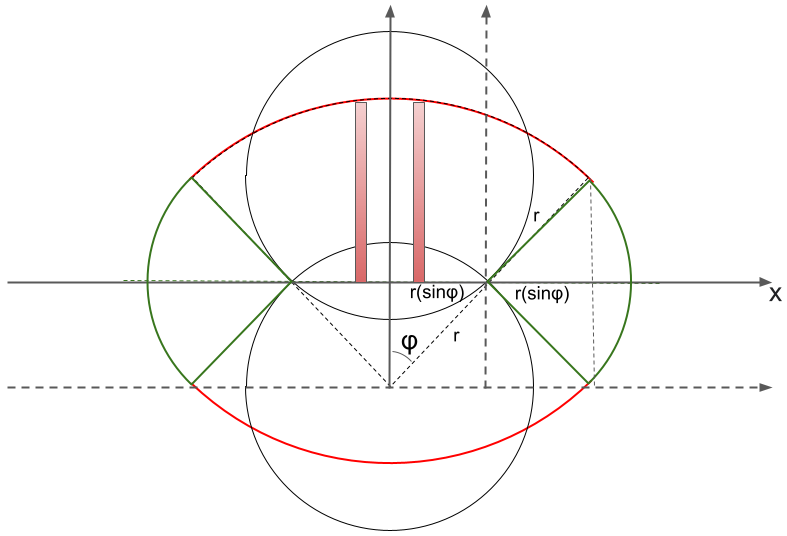
\includegraphics[width=0.45\textwidth]{Cech.png}
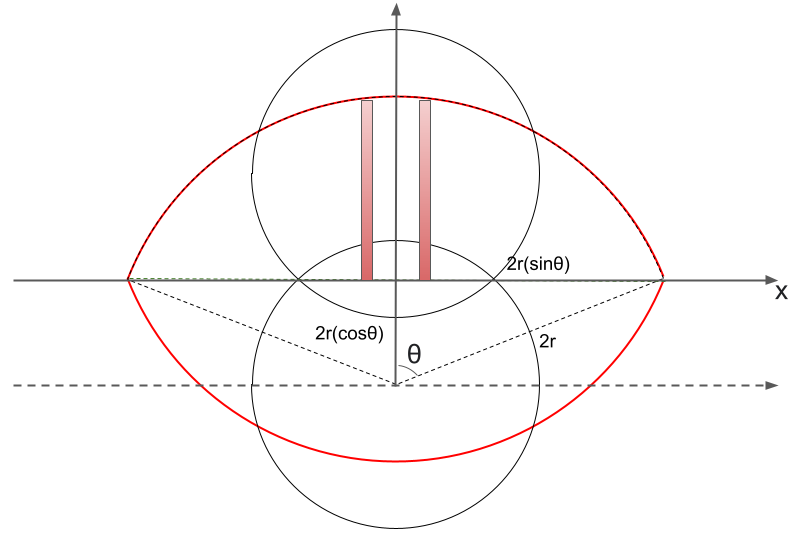
\includegraphics[width=0.45\textwidth]{Rips.png}   
\end{center}

$V_e$ (red, right) is the union of two hyperspherical caps. The caps are of hyperspheres of radius $2r$, whose centers are separated by distance $s$. $[V_e]$ is the product of the volume of a hypersphere with the regularized incomplete Beta function, as follows.

$$
[V_e] = V_d(2r) \cdot I_{\sin^2\phi}\left(\frac{d+1}{2}, \frac{1}{2}\right)
$$

$V_f$ (red and green, left) is the $r$-neighborhood of the union of two small hyperspherical caps. The caps are of hyperspheres of radius $r$, whose centers are separated by distance $s$. (This $r$-neighborhood looks like the overlapping of two large sectors of radius $2r$, plus two small quadrants of radius $r$.) $[V_f]$ is computed parametrically, with the help of the formula for surface area of a 1-dimension-less-hypersphere.

$$
[V_f]= 2\left( \int_0^{\sqrt{1-s^2}} (\sqrt{1-x^2}- \frac{s}{2}) \cdot S_{d-1} \text{ d}x + \int_{0.5\sqrt{1-s^2}}^{0.5} (\sqrt{0.25-x^2}) \cdot S_{d-1} \text{ d}x \right) 
$$

where $S_{d-1}$ refers to the surface area of the $(d-1)$-hypersphere, as follows.

$$
S_{d-1} = \frac{2\pi^{(\frac{d-1}{2})}x^{(d-2)}}{\Gamma(\frac{d-1}{2})}
$$

The above formulae apply to fixed separation distance $s$. To enable us to account for all possible values of $s$, the last ingredient is probability density function for $s$. Putting these together and making $s$ the ratio of the separation distance between the circles' centers and the diameter of the circles, our main result for $q$ follows.

$$
\begin{aligned}
q &= \bigintss_0^{1} \frac{[V_f]}{[V_e]} \cdot ds^{d-1} \text{d}s
\end{aligned}
$$

where $[V_f]$ and $[V_e]$ are below defined.

$$
\begin{aligned}
[V_f]&= 2\left( \int_0^{\sqrt{1-s^2}} (\sqrt{1-x^2}- \frac{s}{2}) \cdot S_{d-1} \text{ d}x + \int_{0.5\sqrt{1-s^2}}^{0.5} (\sqrt{0.25-x^2}) \cdot S_{d-1} \text{ d}x \right) \\
[V_e] &= 2 \left(\int_0^{\sqrt{1-(s/2)^2}} (\sqrt{1-x^2}-\frac{s}{2}) \cdot S_{d-1} \text{ d}x \right) \\
&= V_d(2r) \cdot I_{\sin^2\phi}\left(\frac{d+1}{2}, \frac{1}{2}\right) \\
&= \frac{\pi^{d/2}}{\Gamma(\frac{n}{2}+1)}(2r)^d \cdot I_{\sin^2\phi}\left(\frac{d+1}{2}, \frac{1}{2}\right)
\end{aligned}
$$

where $I_{\sin^2\phi}$ refers to the regularized incomplete beta function, as follows.

$$
I_z(a,b) = \frac{\int_0^z u^{(a-1)}(1-u)^{(b-1)}  \text{ d}u}{\int_0^1 u^{(a-1)}(1-u)^{(b-1)} \text{ d}u}
$$

\newpage
\section{Leading Order Asymptotics for q}

We reason that the leading order asymptotic behaviour of $q$ depends on $d$, the ambient dimension. We first determine the dependence of $[V_e]$ on $d$. For fixed separation $s$, this depends on the regularized incomplete beta function $I_{\sin^2\phi}\left(\frac{d+1}{2}, \frac{1}{2}\right)$. For general $s$, we multiply $I_{\sin^2\phi}\left(\frac{d+1}{2}, \frac{1}{2}\right)$ by the probability density function of $s$ as determined by ambient dimension $d$.

$$
\begin{aligned}
\text{pdf }(s) &= \dfrac{d}{ds} \left(s^d\right) \\
&= ds^{d-1}
\end{aligned}
$$

This gives us the following integral, which we have yet to calculate.

$$
\begin{aligned}
    \E [V_e] &= \bigintsss_0^{1} I_{\sin^2\phi}\left(\frac{d+1}{2}, \frac{1}{2}\right) \cdot ds^{d-1} \text{ d}s \\
    &= \text{ (to be found)}
\end{aligned}
$$

We will consider the difference in volume between $[V_f]$ and $[V_e]$, which we call $[V_x]$. To calculate $[V_x]$ in arbitrary dimension, we need to multiply $[V_x]$ by $S_{d-1}$ according to the method of shells in calculating volumes of revolution.

\begin{center}
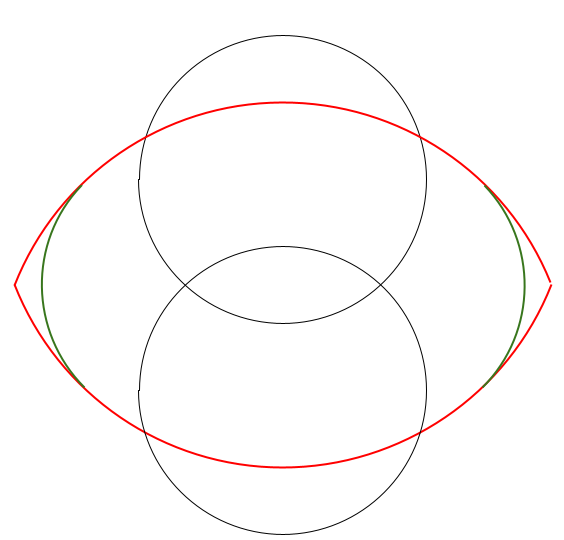
\includegraphics[width =0.45 \textwidth]{Compare.png}    
\end{center}

$$
\begin{aligned}
    [V_x] &= \text{ to be found in terms of }s \\
    \E [V_x] &= \bigintsss_0^{1} [V_x] \cdot  S_{d-1} \text{ d}s \\
    &= \text{ (to be found)}
\end{aligned}
$$

Then we will have $q = \frac{V_e - V_x}{V_e}$.

\section{Numerical analysis of q}

While a closed form expression and leading order asymptotics for $q$ are still in progress, $q$ is seen to decrease with respect to ambient dimension in the following plot.

\begin{center}
    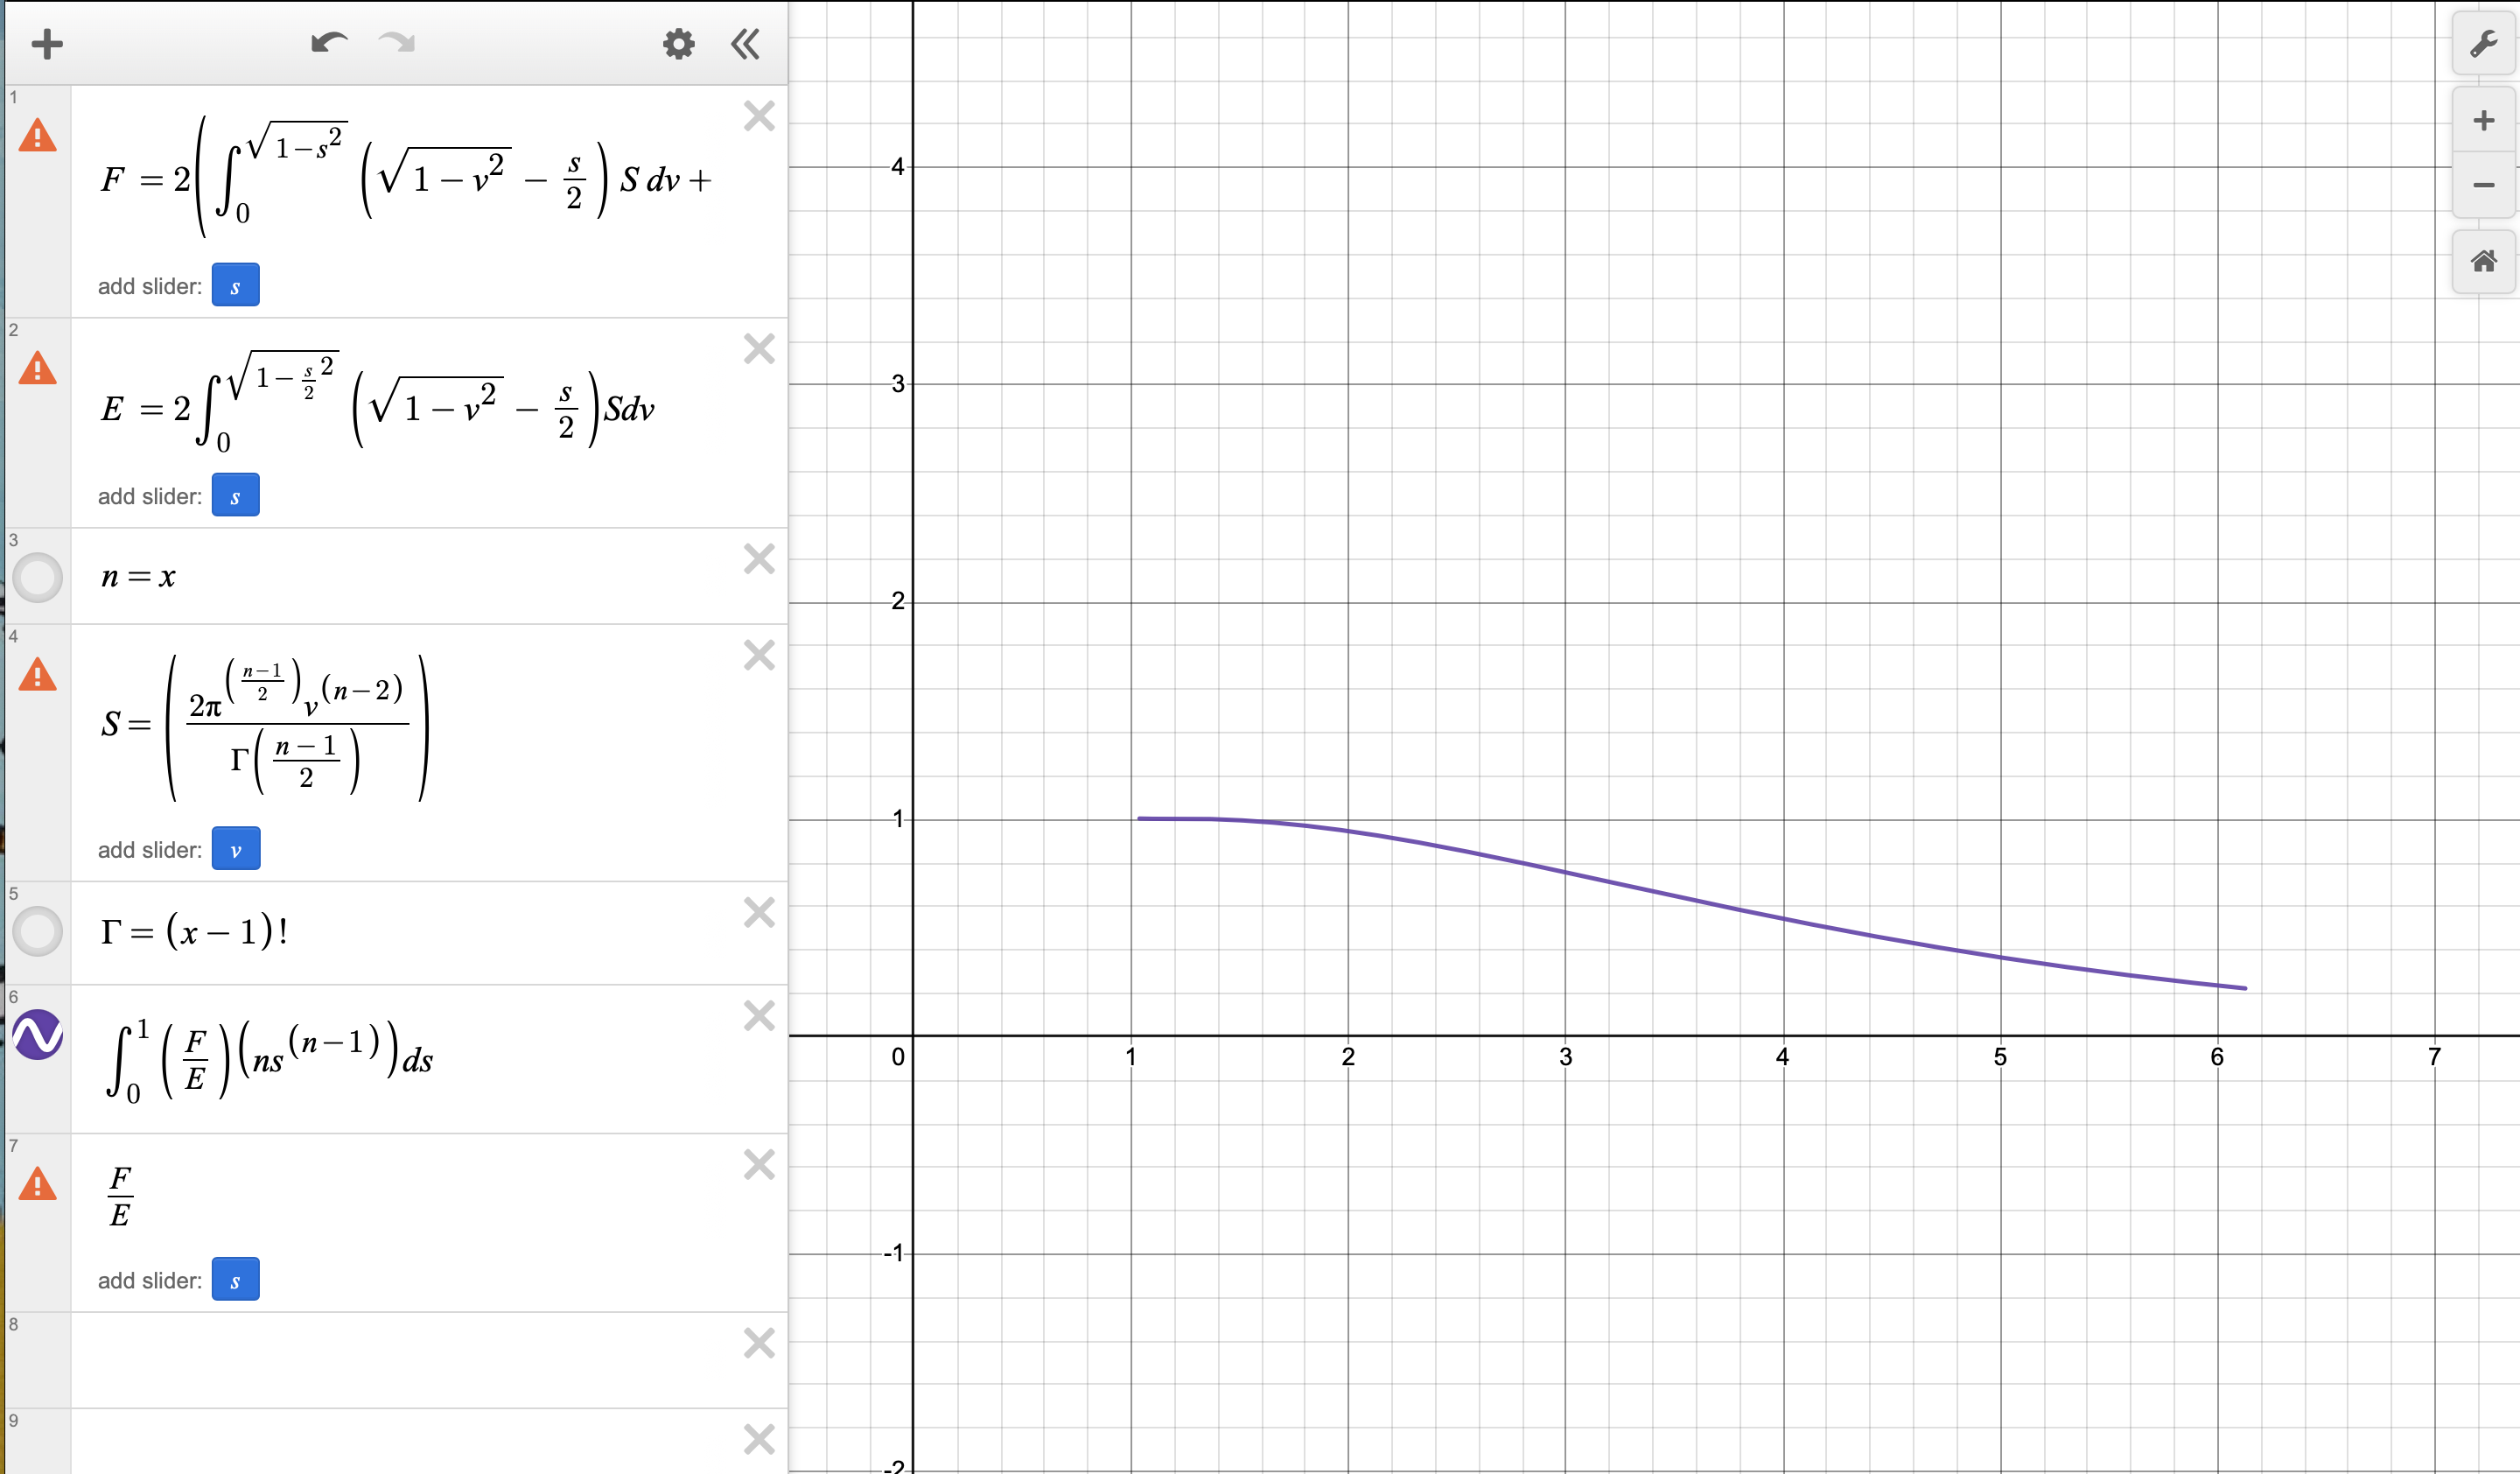
\includegraphics[width=0.7\textwidth]{q.png}
\end{center}

\section{Expectation and Variance of Filled Triangles in Čech complex in space of ambient dimension $d$}

\subsection{$\E[\Delta_f]$ in Čech complex of dimension $d$}

We want to find $\P(\Delta_f)$ in terms of $p$, the edge-adding probability. First letting the ambient space have volume 1, we have $p = V_d(2r)$. Inverting the volume formula, we have  

$$
r = \frac{\Gamma(\frac{n}{2}+1)^{1/d}}{2\sqrt{\pi}}p^\frac{1}{d}
$$

Now we adapt our calculation of $[V_f]$ to get $\P(\Delta_f | s < 2r)$.

$$
[V_f](r,s) = 2\left(\int_0^{2r\sin\phi}(\sqrt{1-x^2}-2r\cos\theta)\cdot S_{d-1} \text{ d}x + \int_{r\sin\phi}^r(\sqrt{r^2-x^2}\cdot S_{d-1}\text{ d}x \right)
$$

We let $t = \frac{s}{2r}$ and integrate over $t \in [0,1]$, the equivalent of integrating $s$ from $0$ to $2r$. Recalling that $\phi = \arccos (\frac{s}{2r}) = \arccos t$ and $\theta = \arccos (\frac{s}{4r}) = \arccos (\frac{t}{2})$, and the probability density function of $t$, we have 

$$
\begin{aligned}
\P(\Delta_f | s < 2r) &= \E[[V_f](r)] \\
&= \int_0^1 \left[ V_f(r,t) \right] \text{pdf}(t) \text{ d}t \\
&= \int_0^1 \left[ \int_0^{2r\sqrt{1-t^2}} \left( \sqrt{1-x^2} - rt \right) \cdot S_{d-1} \text{ d}x + \int_{r\sqrt{1-t^2}}^r \left( \sqrt{r^2-x^2} \right) \cdot S_{d-1} \text{ d}x \right] 2t \text{ d}t
\end{aligned}
$$

Substituting $r(p)$ above, gives $\P(\Delta_f | s<2r)$, and so:
$$
\begin{aligned}
\P(\Delta_f) &= \P(\Delta_f | s<2r)\P(s<2r) \\
&= p \cdot \E[[V_f](p)]  
\end{aligned}
$$
where $r$ has been replaced by the function of $p$ given above. 

By linearity of expectation:
$$
\E[\Delta_f]= {n \choose 3} \P(\Delta_f)
$$

\subsection{Var$[\Delta_f]$ in Čech complex}

In this section, $\E[[V_f]]$ is a function of $p$. Parallel to what we had in Section 5, and this time using $I_f$ as the indicator of a filled triangle:

$$
\begin{aligned}
\mathbb{E}[\Delta_f] &= {n \choose 3} \P(I_f | s<2r)\P(s<2r) \\
\mathrm{Var}[\Delta_f] &= {n \choose 3} \mathrm{Var}(I_f) + 12 {n \choose 4} \mathrm{Cov}(I_{f1}I_{f2}) 
\end{aligned}
$$

This is because:

$$
\mathrm{Var}(\Delta_{f})=\mathrm{Var}\left(\sum I_{f}\right)=\sum \mathrm{Var}\left(I_{f}\right)+\sum_{f1 \neq f2} \mathrm{Cov}\left(I_{f1} I_{f2}\right)
$$

The only way that the triangles be dependent is if they share 1 edge. Counting the ordered pairs of triangles that share an edge, note that any such pair has four vertices, and each set of four vertices corresponds to twelve such pairs (any one of the edges can be the shared one, and then two orders). \hyperlink{https://math.stackexchange.com/questions/2736641/variance-in-the-number-of-triangles-in-a-random-graph-of-size-n}{(Source)}

$$
\begin{aligned}
\mathrm{Var}\left( I_{f}\right) &= \P(I_{f}) (1-\P(I_{f})) \\
&= p \cdot \E[[V_f]] (1-p \cdot \E[[V_f]]) \\
\mathrm{Cov}(I_{f1}I_{f2}) &= \E[I_{f1}I_{f2}] - \E[I_{f1}]\E[I_{f2}]  \\
&= p \cdot \E[[V_f]]^2 - (p \cdot \E[[V_f]])^2 \\
&= (p-p^2) \cdot \E[[V_f]]^2
\end{aligned}
$$
Hence,
$$
\begin{aligned}
\E[\Delta_f]&= {n \choose 3} p \cdot \E[[V_f]]  \\
\mathrm{Var}[\Delta_f] &= {n \choose 3} \mathrm{Var}(\Delta_f) + 12 {n \choose 4} \mathrm{Cov}(\Delta_{f1}\Delta_{f2}) \\
&= {n \choose 3} \left( p \cdot \E[[V_f]] (1-p \cdot \E[[V_f]])\right) + 12 {n \choose 4} \left( (p-p^2) \cdot \E[[V_f]]^2 \right)
\end{aligned}
$$

\subsection{Leading Order Asymptotics}

The variance in the number of filled triangles is of a very similar form in both 2PC and Čech. To get the Var in Čech, substitute every $p^3q$ in Var in 2PC with $p \E[V_f]$.

$\P(\Delta_f | s<2r) = \E[[V_f]]$ proves extremely time-consuming to compute. However, we conclude the following numerically:

By removing the upper-half-cap to simplify the computation and restricting the ambient dimension to 3 (and matching $q$ = 0.757), we can verify that variance of the filled triangle statistic is much higher in the Čech complex than the 2-parameter Erdös-Renyi. Moreover, the $n^4$ term dominates the variance in both complexes. 

\begin{center}
    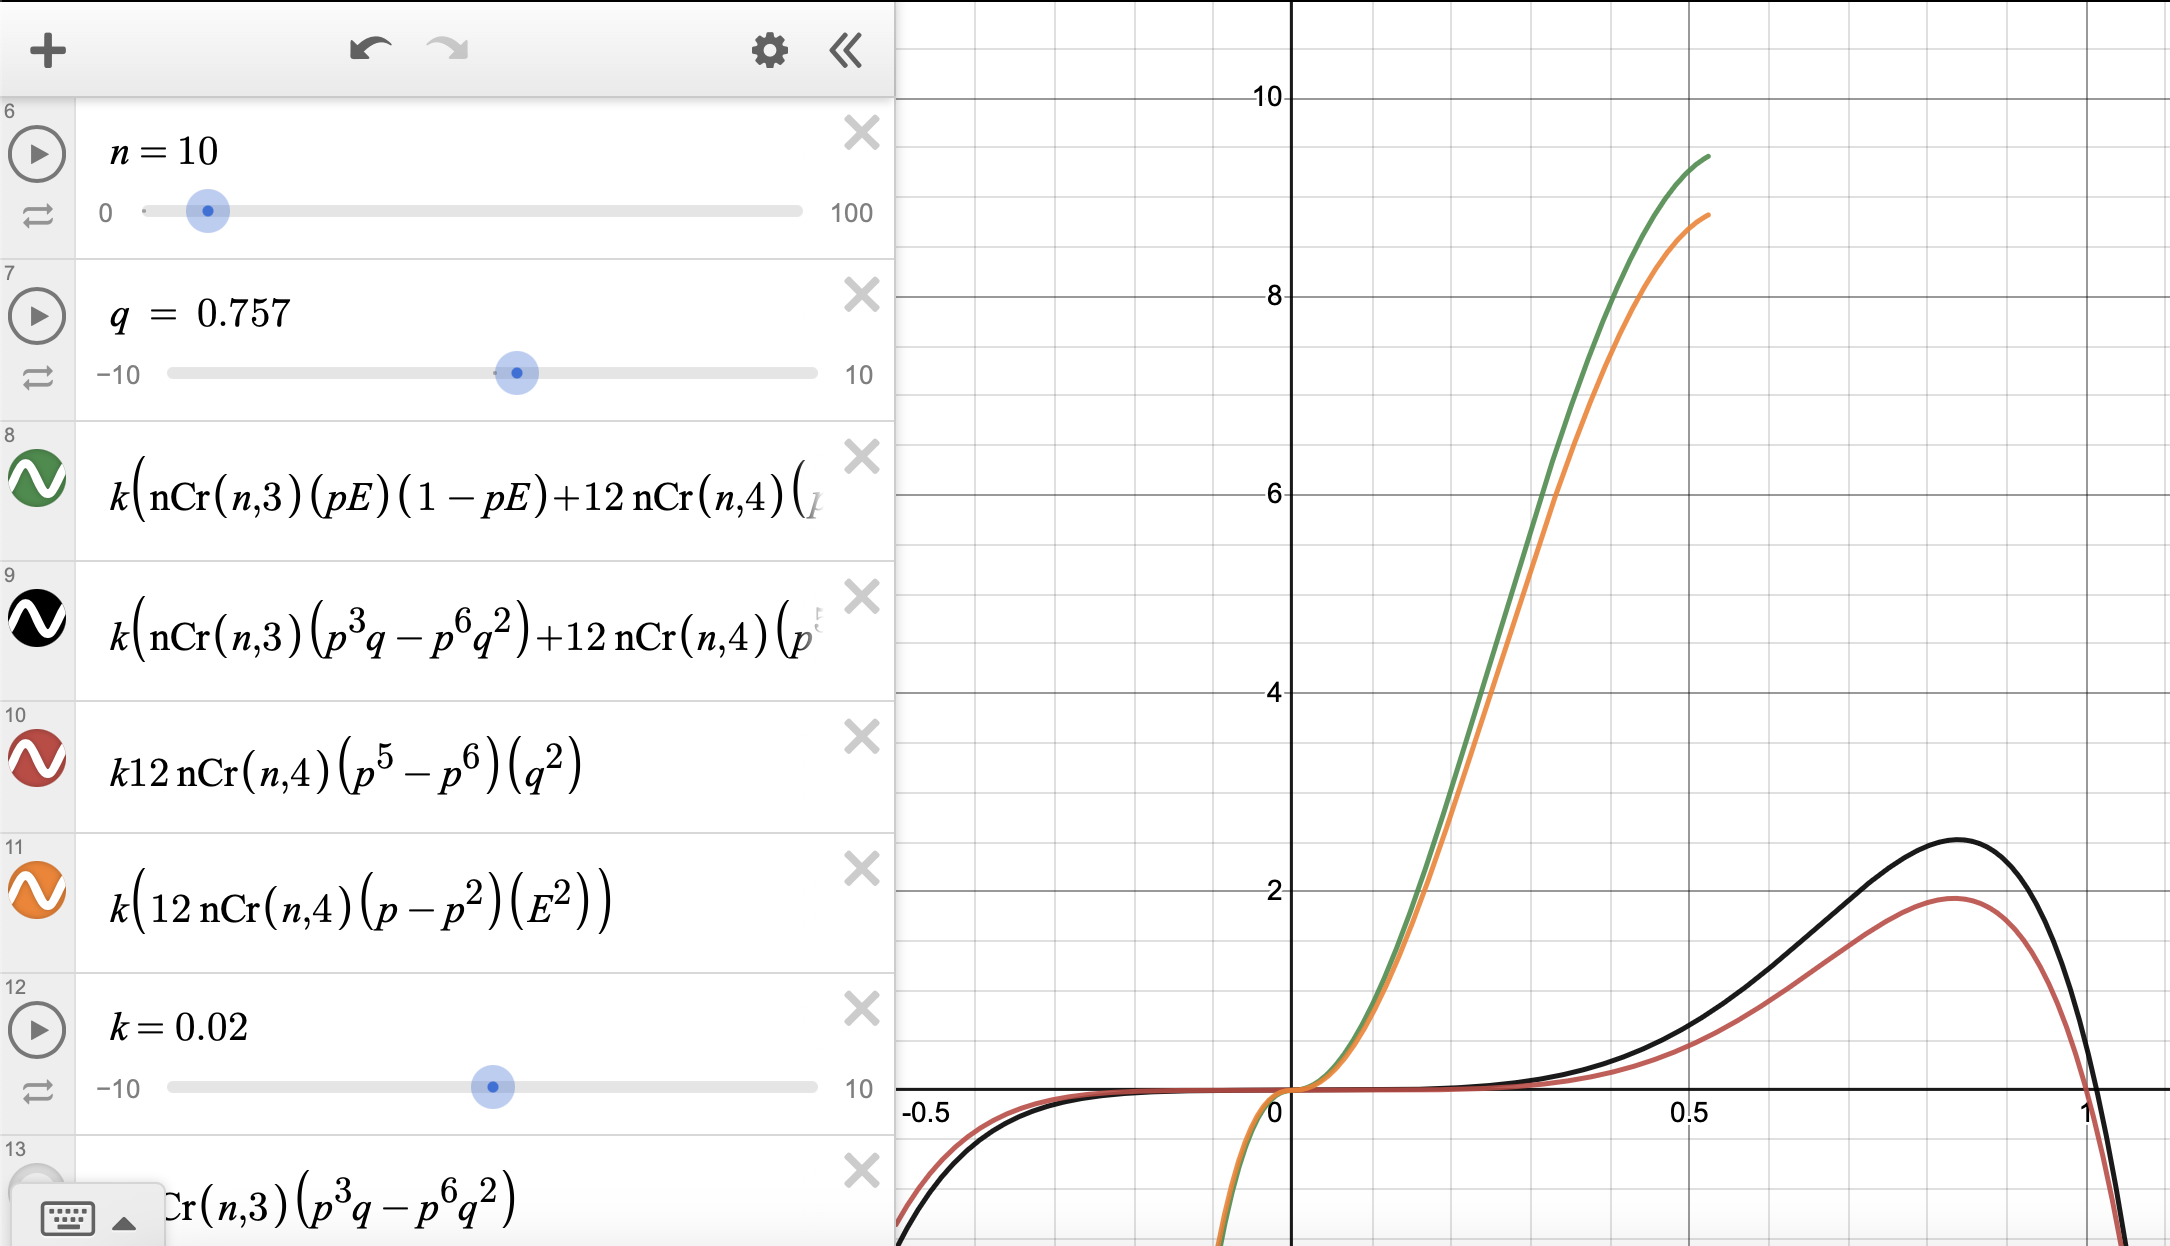
\includegraphics[width=0.5\textwidth]{Variance Comparison.png}
\end{center}

Removing the upper-half-cap and computing in general dimensions, we observe that $\P(\Delta_f | s<2r)$ is defined for dimensions below $n_{\log p}$ where the upper bound appears to be a logarithmic function of $p$. Higher dimensions are only computable for extremely small $p$.

The difference in the expected number of filled triangles is ${n \choose 3} (\E[[V_f]] - p^2)$. At least for dimensions 1 through 4, it is obvious from the plots that this difference is non-negligible.

\begin{center}
    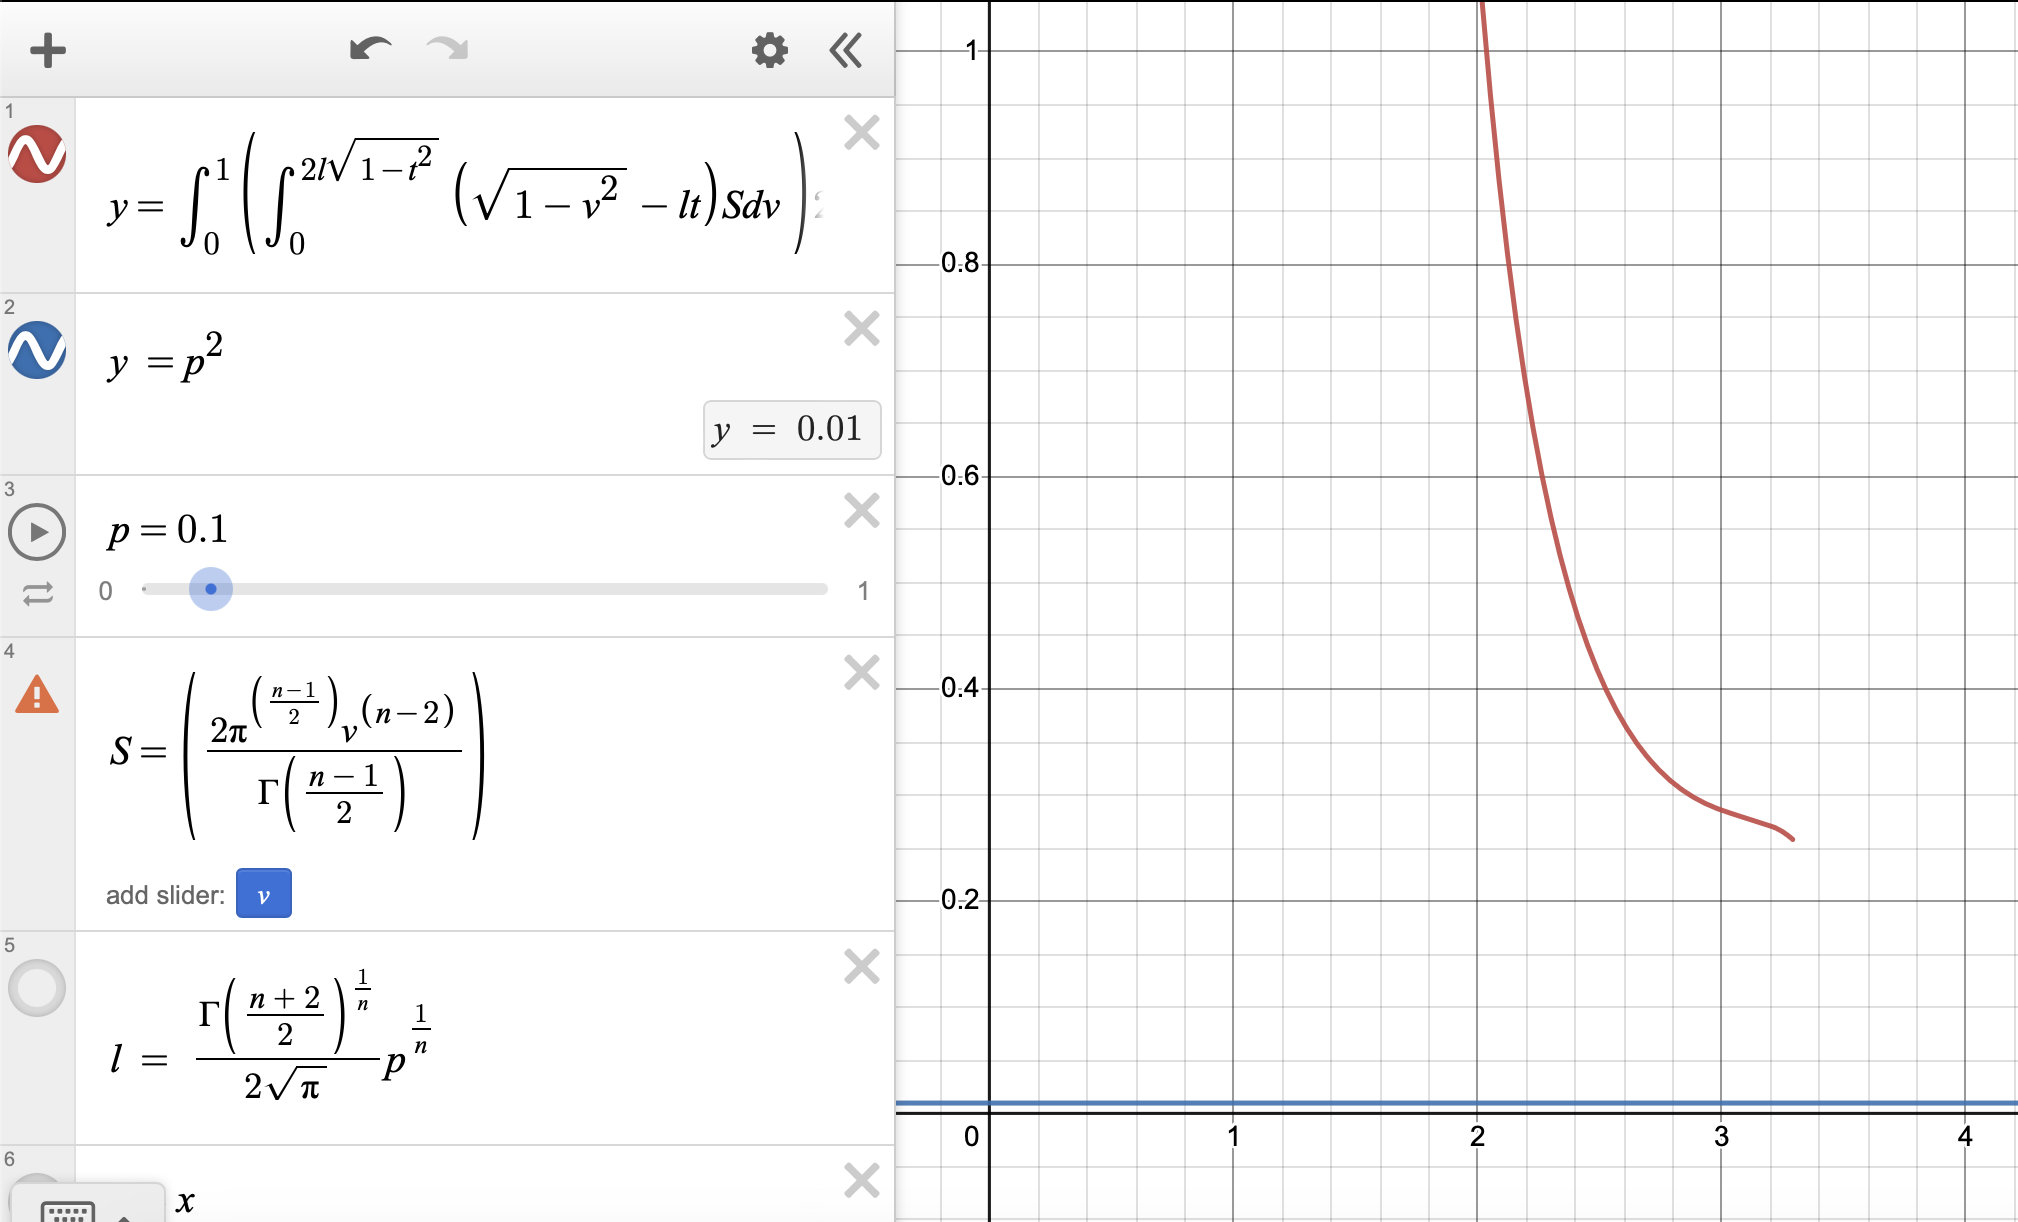
\includegraphics[width=0.3\textwidth]{Comparing Expectation1.png}
    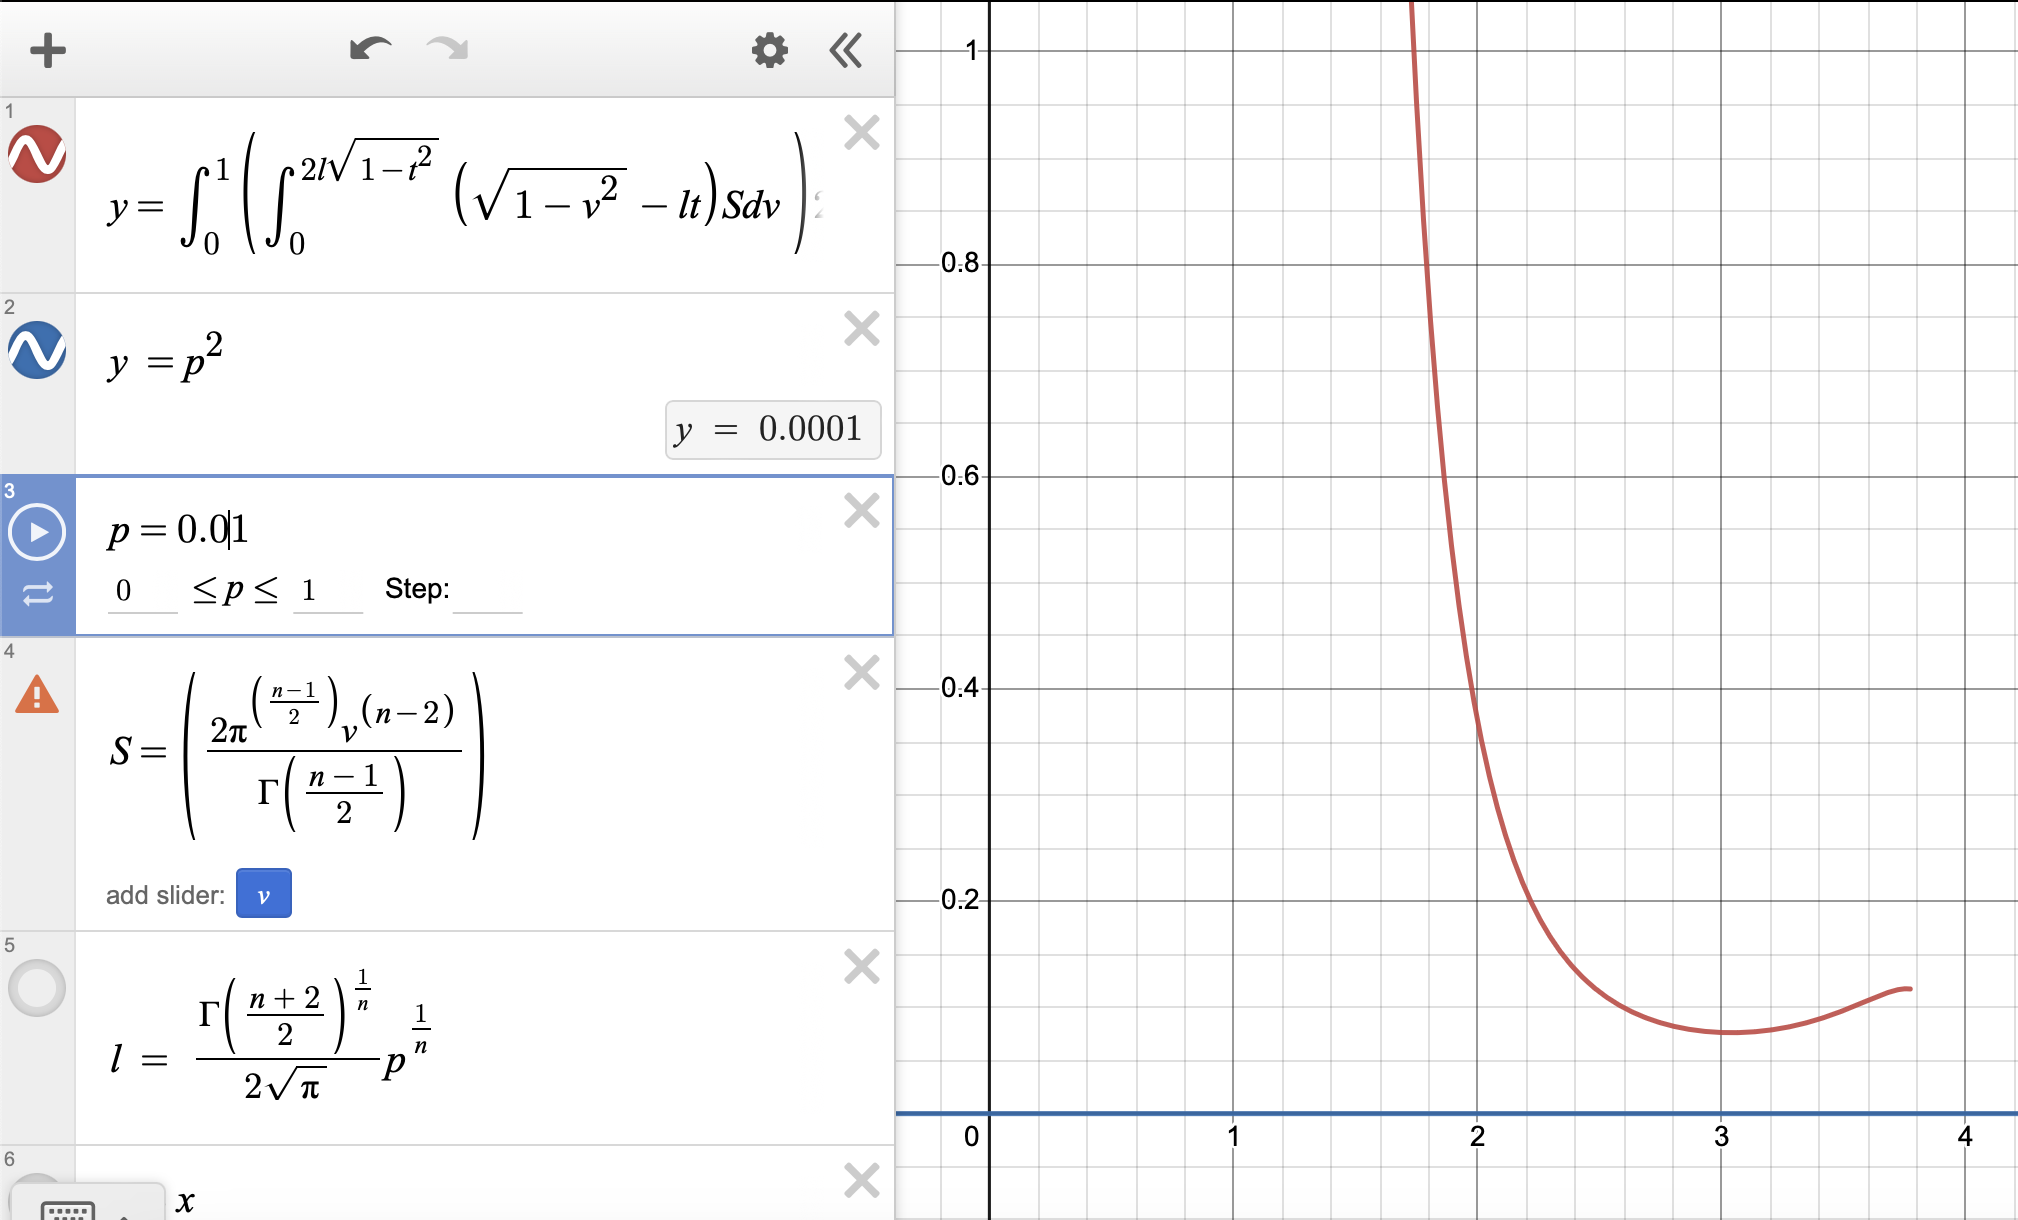
\includegraphics[width=0.3\textwidth]{Comparing Expectation2.png}
    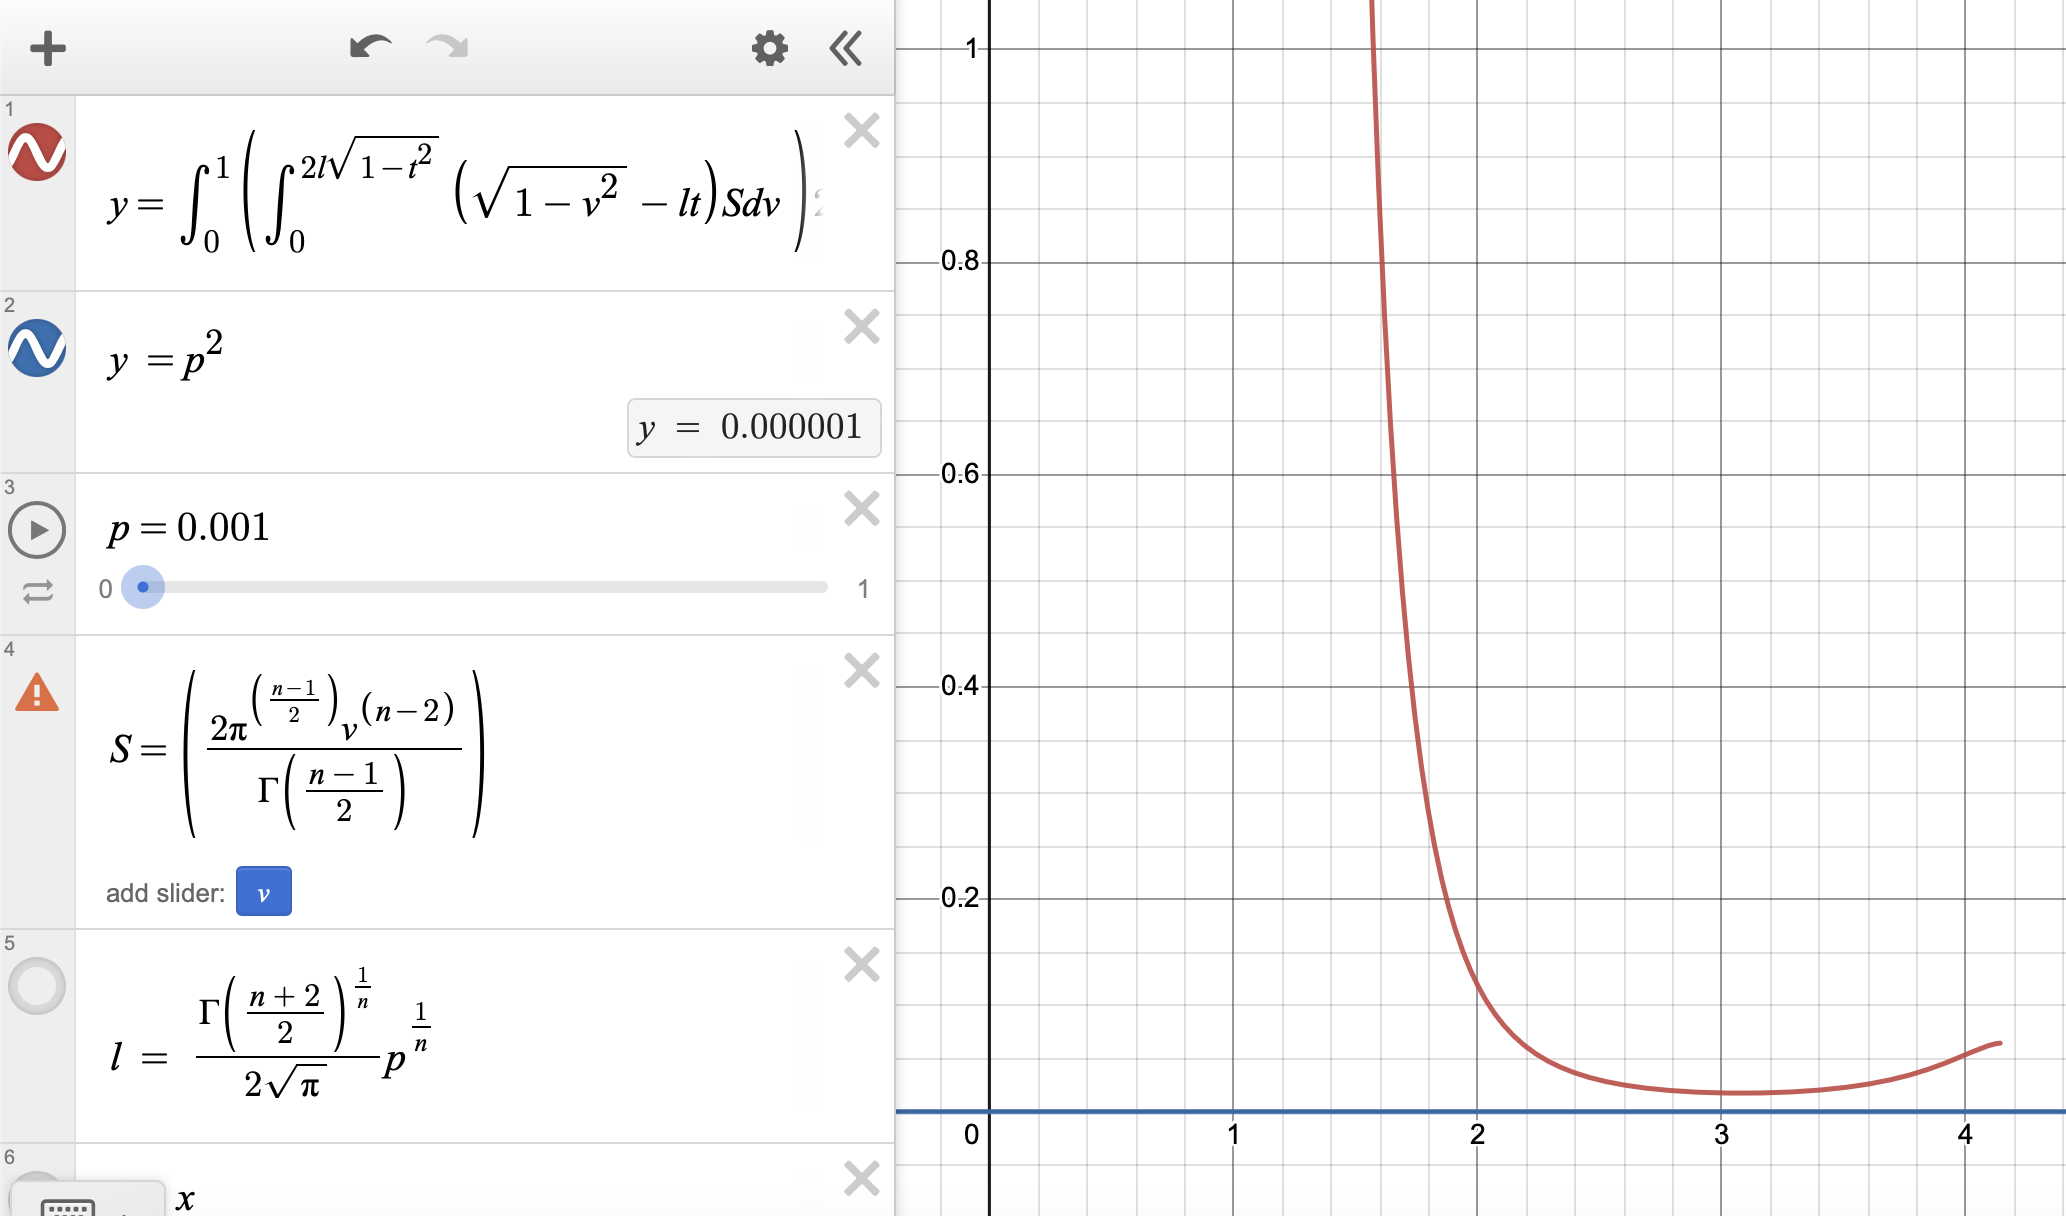
\includegraphics[width=0.3\textwidth]{Comparing Expectation3.png}
\end{center}

Asymptotically we see $\E[\Delta_f]$ to be on the order of $n^3p \E[V_f]$ while $\mathrm{Var}(\Delta_f)$ is on the order of $n^4(p-p^2)(\E[V_f])^2$. The former dominates the latter when:

$$
\frac{n^3pE}{n^4(p-p^2)E} = \frac{1}{n(1-p)E} \rightarrow \infty.
$$

and testing becomes impossible when:

$$
\frac{1}{n(1-p)E} \rightarrow 0
$$

Where $E= \E[V_f]$ has yet to be described in terms of how it behaves with respect to $p,d$. 

\section{Next steps}

In our Fall 2023 independent study, we will derive leading order asymptotics for the above expressions and so concretize the answer to the power of the filled triangle statistic. We will then use other substructures, such as the "flapwheel" substructure, to see if they yield statistics with greater power than the "filled triangle".

\end{document}